\section{Theory}\anote{Da cambiare}
\label{sec:theory}

\fboxsep=1mm%padding thickness
\fboxrule=1pt%border thickness

\begin{figure*}[!ht]
	\centering
		%  trim={<left> <lower> <right> <upper>}
        %\fcolorbox{red}{yellow}{
            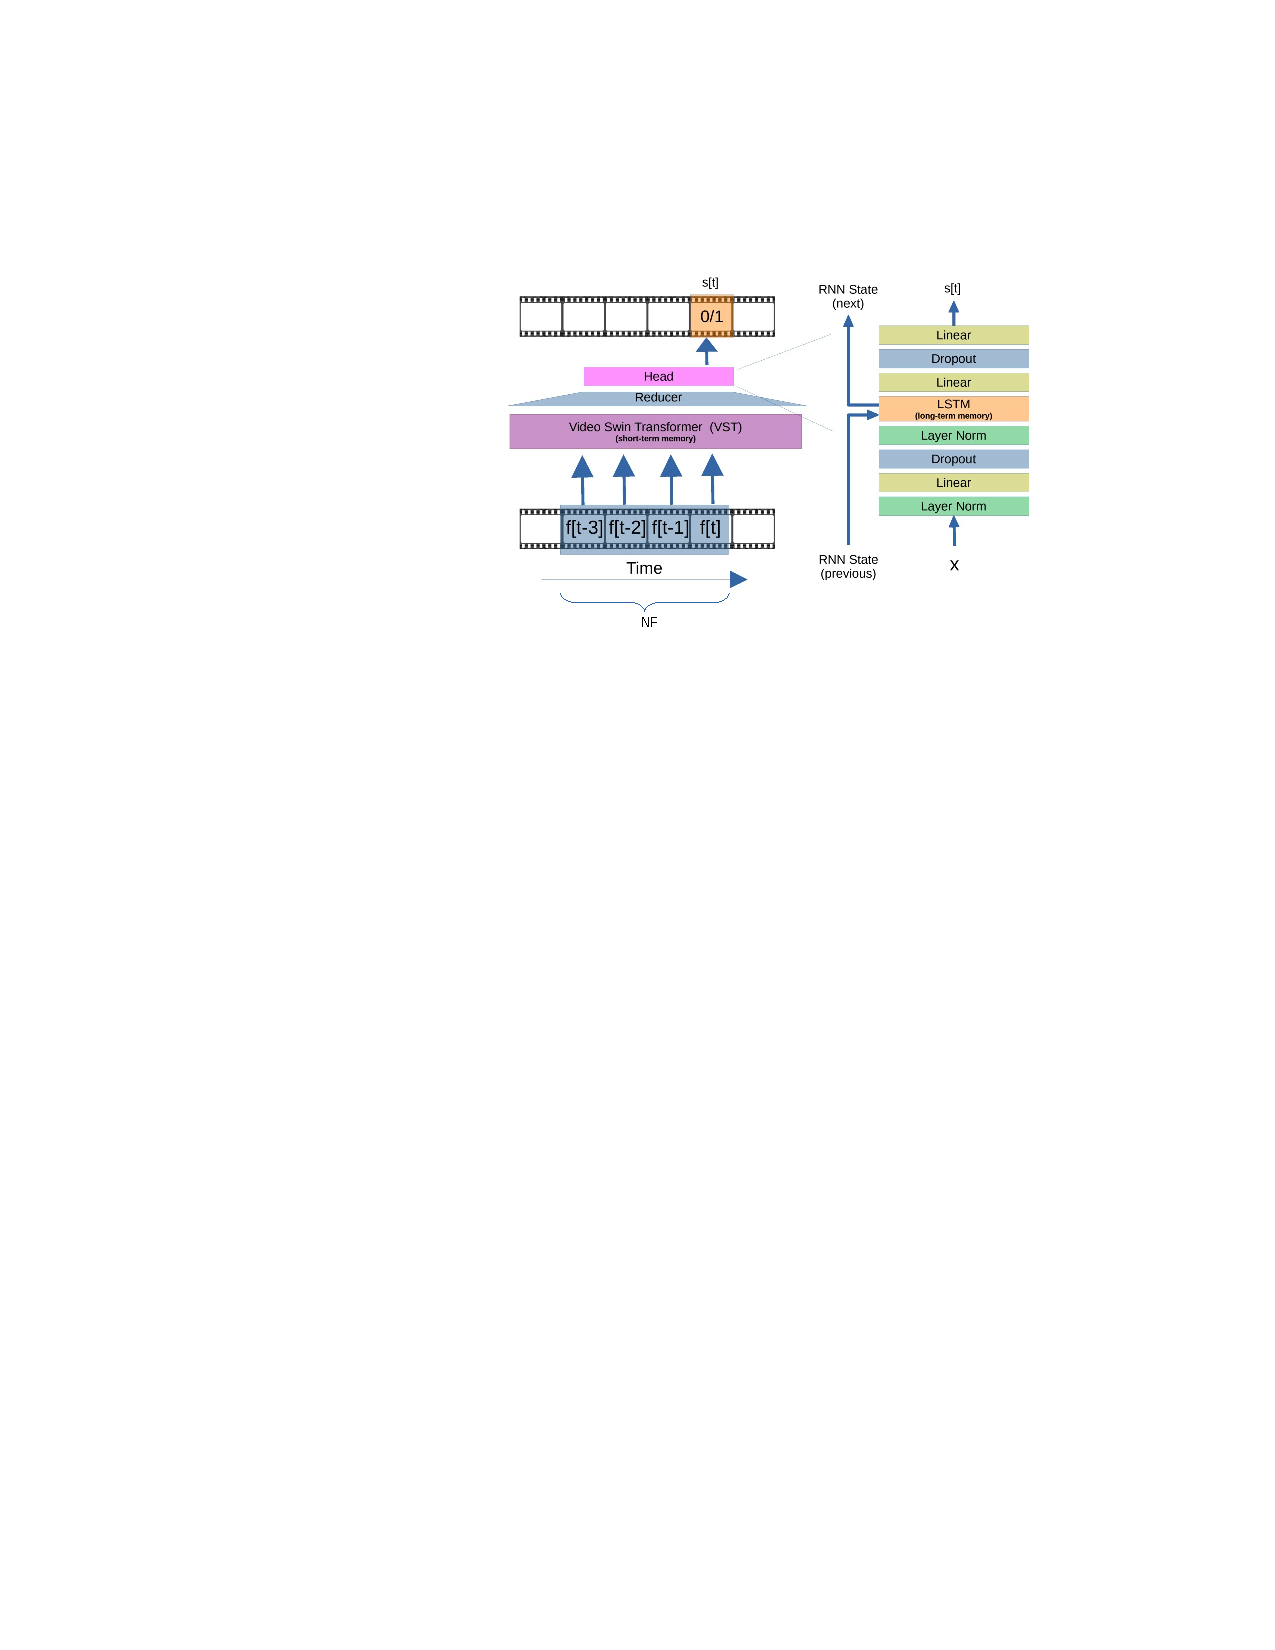
\includegraphics[trim=205 500 80 130, clip, width=1.\linewidth]{images/arch.pdf}
        %}
        % FIXME aggiungi link per immagine dei frame (copyright)
        \caption{Our online video frame anomaly detection architecture. $f[t]$ is the frame at time $t$, $x$ the output of the Reducer.}
		\label{fig:arch}
\end{figure*}

In this section, the overall architecture shown in Figure~\ref{fig:arch} will be explained.
The model is composed by four main blocks: a short-term memory module to encode the information related to what is happening in the present and the near past, a long-term memory module to also keep track of the remote past and the final classification module. \anote{Evidenzierei poi nella nuova versione della Fig. 1 i 4 blocchi di cui si parla qui}
% TODO descrivere la nuova annotazione ??? Check motivazioni! :)

\noindent\textbf{Short-term memory}
%TODO Breve accenno su tranformer MB: SECONDO ME NON CI STA
Taking inspiration from \cite{xu2021long}, recently observed frames have been taken into account as a source of information related to the ongoing action, and past frames as a source of information on the context.
Since the task requires an online anomaly frame classification, it means the only information available are the current and the past frames.
At each step, the chosen number of processed frames is three (the current one and the previous two frames).
Experiments will report an ablation study to justify this specific choice.\lnote{check, perchè 4 sembra meglio!}
The network has to take the time into consideration, as incorrect behavior is often recognizable by taking into consideration the immediate past.
To model short memory, we selected a Vision Transformer \cite{DBLP:conf/iclr/DosovitskiyB0WZ21} solution, which has become very popular in computer vision tasks, challenging the predominance of CNN architectures.
The transformer model was chosen over an RNN given the ability to process frames in parallel.
In particular, the Video Swin Transformer (VST) \cite{liu_video_2022} was chosen as the basic model due to its superior performance compared to a vanilla ViT \cite{DBLP:conf/iclr/DosovitskiyB0WZ21} model.
The VST model is the extension to video of the Swin Transformer \cite{liu2021Swin}, which is a general-purpose image backbone with high performance on tasks that involve detection and localization.
Originally born to carry out the task of video action classification, analyzing all the frames in one step, it has been adapted in this work to detect anomalies on single frame at time $t$, in a near-real time fashion, considering a temporal window of the latest three frames at time $t-2$, $t-1$ and $t$.

VST takes as input a video with size $T \times H \times W \times 3$, where $T$, $H$ e $W$ correspond to number of frames, height, width and channels RGB, respectively.
The model internally splits the frames in non-overlapping 3D patches, partitioning the video in $\frac{T}{2} \times \frac{H}{4} \times \frac{W}{4}$ 3D tokens, projecting the features to an arbitrary dimension $C$.
The rest of the architecture is similar to Swin Transformer, with four stages of Video Swin Transformer block, interspersed with $2\times$ spatial downsampling in the patch merging layer.
As shown in Figure \ref{fig:arch}, in our case $T=3$, i.e., the input of the VST is formed by $f[t-2]$, $f[t-1]$ and $f[t]$, where $f[y]$ represents the frame at time $y$.

\noindent\textbf{Classification module (Head).}
After reducing the output of the VST with a Adaptive Average Pool 3D (called Reducer in Fig. \ref{fig:arch}), the classification module processes it, generating the final output.
For each frame at time $t$, the final output is the anomaly classification score $s_t \in [0,1]$, where $s_t=0$ means absence of anomaly and $s_t=1$ means the frame is surely anomalous.
This is trained with a weighted cross-entropy loss, giving more weight to the anomaly class, because it is spotted less frequently \tnote{scriviamo il rapporto fra le due classi: 70/30?} \vnote{TODO: contare il numero effettivo di frame anomali/normali}.
As shown in Figure \ref{fig:arch}, the head is composed by some layers normalization, linear layers and dropout, alternating. 
In between, the LSTM cells are introduced to implement our long-term memory.

%train  dataset:  3191  video annotations found
%Normal frames found:  221429
%Anomaly frames found: 108121
%val  dataset:  1376  video annotations found
%Normal frames found:  94347
%Anomaly frames found: 46971

\noindent\textbf{Long-term memory.}
In order to not lose information from the distant past, we needed a way to keep track of it.
Because the model is working in an online fashion and each frame is taken into account in the exact moment when is available, the requirements are opposite compared to the short-term memory.
We update the long-term memory sequentially, when a new frame is available.
For this reason, our choice fell on an RNN module (LSTM in this specific case) instead of a Transformer.
Because it does not need to access the past frames again, but only the latent features, the module is very efficient and lead to a limited additional computational cost.
Indeed, it condenses all its knowledge into two states: an hidden state $h_t$ and cell state $c_t$.
Since the output of the first Linear layer of the classifier head provides the summary about the three frames processed by the short-term memory model, the LSTM cells is added immediately after updating the memory states with the new information.
\vnote{specificare che le celle LSTM sono stacked qui o in experiments}

% copyright image frame: <a href="https://www.freepik.com/free-vector/realistic-vector-icon-film-tape-strip-with-white-square-isolated-white-cinema-concept_31096470.htm#query=video%20frame&position=31&from_view=keyword">Image by user15245033</a> on Freepik